\documentclass[25pt, portrait, margin=2cm, colspace=2cm, blockverticalspace=1.5cm]{tikzposter}
\usepackage[utf8]{inputenc}
\usepackage{graphicx}
\usepackage{amsmath}
\usepackage{qrcode}
\usepackage{hyperref}

% --- Custom UPenn Academic Color Scheme ---
\usetheme{Default} 
\definecolor{PennBlue}{RGB}{1, 31, 91}
\definecolor{PennRed}{RGB}{153, 0, 0}

% Apply colors to poster elements
\colorlet{backgroundcolor}{white}
\colorlet{titlebgcolor}{PennBlue}
\colorlet{titlefgcolor}{white}
\colorlet{blocktitlebgcolor}{PennBlue}
\colorlet{blocktitlefgcolor}{white}
\colorlet{blockbodybgcolor}{white}
\colorlet{blockbodyfgcolor}{black}

% Remove the default TikZposter watermark at the bottom right
\tikzposterlatexaffectionproofoff 

% --- Title Block ---
% Added negative vspace to shrink the wasted blue padding at the top and bottom
\title{\vspace{-1cm}\parbox{\linewidth}{\centering {\Huge \textbf{Scalable Multi-Robot Coordination:}} \\
{\LARGE Integrating LCBA Task Allocation with Decentralized Path Planning}}}
\author{Shreyas Raorane}
\institute{{\Large Master of Science in Engineering in Robotics, University of Pennsylvania}\\[4pt]
{\Large Advisors: Dr. Linh Thi Xuan Phan, Dr. Rahul Mangharam, Dr. Ani Hsieh}\vspace{-1cm}}

\begin{document}

\maketitle

\begin{columns}

% ==========================================
% COLUMN 1 (LEFT)
% ==========================================
\column{0.5}

\block{1. The Problem Context}{
    \textbf{Context:} Modern warehouse fleets require dynamic Multi-Robot Task Allocation (MRTA) to operate efficiently. \\[4pt]
    \textbf{The Flaw:} Consensus algorithms (CBBA, GCBBA) assume global connectivity or static links. \\[4pt]
    \textbf{The Reality:} Range-limited radios, obstacles, and agent mobility produce dynamic partitions; baselines can fail to reach consensus and stall operation.
}

\block{2. The Solution: LCBA}{
    The \textbf{Local Consensus-Based Bundle Algorithm (LCBA)} relaxes the global connectivity assumption.
    \begin{itemize}
        \item \textbf{Component-local consensus:} Bidding and consensus operate within each current connected component.
        \item \textbf{Dynamic resolution:} Time-stamped allocations resolve conflicts on reconnection.
        \item \textbf{Event-driven replanning:} Supports continuous task arrivals without full a priori knowledge.
    \end{itemize}
}

\block{3. System Architecture}{
    \begin{center}
        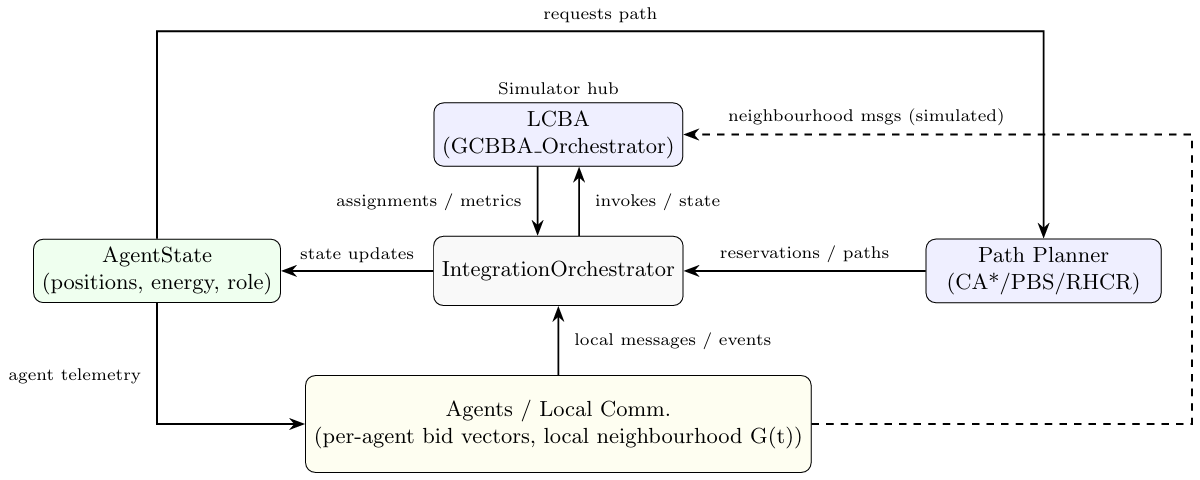
\includegraphics[width=0.9\linewidth, height=26cm, keepaspectratio]{figures/system_architecture.png}
        \vspace{0.1cm}
        {\textbf{Figure:} System Architecture integrating LCBA with role-based planners.}
    \end{center}
    \vspace{0.1cm}
    \textbf{Design:} Logically decentralized allocation (LCBA) integrates with role-based path planners (CA*, PBS, RHCR) to ensure collision-free execution.
}

\block{4. Experimental Scale}{
    Developed a discrete-time gridworld simulator to evaluate algorithmic limits.
    \begin{itemize}
        \item \textbf{Scale:} 432 experimental runs across 6 maps.
        \item \textbf{Agents:} Up to 200 agents.
        \item \textbf{Evaluation:} Batch (makespan) and steady-state (throughput) regimes.
    \end{itemize}
}

\block{Simulation Environments}{
    \begin{center}
        \begin{minipage}[t]{0.31\linewidth}
            \centering
            % Swap with your first map (e.g., warehouse_small)
            \includegraphics[width=\linewidth, height=12cm, keepaspectratio]{example-image-a}
            \vspace{0.2cm} \\
            {\textbf{1.} \texttt{warehouse\_small}}
        \end{minipage}\hfill
        \begin{minipage}[t]{0.31\linewidth}
            \centering
            % Swap with your second map (e.g., crossdock)
            \includegraphics[width=\linewidth, height=12cm, keepaspectratio]{example-image-b}
            \vspace{0.2cm} \\
            {\textbf{2.} \texttt{crossdock}}
        \end{minipage}\hfill
        \begin{minipage}[t]{0.31\linewidth}
            \centering
            % Swap with your third map (e.g., warehouse_large)
            \includegraphics[width=\linewidth, height=12cm, keepaspectratio]{example-image-c}
            \vspace{0.2cm} \\
            {\textbf{3.} \texttt{warehouse\_large}}
        \end{minipage}
    \end{center}
}

% ==========================================
% COLUMN 2 (RIGHT)
% ==========================================
\column{0.5}

\block{5. Batch Regime: Communication Robustness}{
    \begin{center}
        % Increased height to 22cm to fill the recovered space
        \includegraphics[width=0.9\linewidth, height=22cm, keepaspectratio]{example-image-b}
        \vspace{0.1cm}
        {\textbf{Figure:} Batch regime completion rate heatmap (warehouse large).}
    \end{center}
    \vspace{0.1cm}
    \begin{itemize}
        \item \textbf{Survival:} LCBA achieves non-zero task completion at \textit{all} tested communication ranges, including fully disconnected states ($\le$ 4 grid units).
        \item \textbf{Baseline Failure:} Under identical conditions, baselines (CBBA, SGA) experience 100\% timeout failure.
        \item \textbf{Optimality:} Maintains a $0.91\times$ makespan ratio relative to greedy centralized assignment on connected graphs.
    \end{itemize}
}

\block{6. Steady-State Regime: Sustaining Throughput}{
    \begin{center}
        % Increased height to 22cm to fill the recovered space
        \includegraphics[width=0.9\linewidth, height=22cm, keepaspectratio]{example-image-c}
        \vspace{0.1cm}
        {\textbf{Figure:} Steady-state capacity frontier across all maps.}
    \end{center}
    \vspace{0.1cm}
    \begin{itemize}
        \item \textbf{Flat Profile:} LCBA maintains a flat, near-peak throughput profile across the entire connectivity spectrum.
        \item \textbf{Saturation Behavior:} Baseline throughput collapses by over 15\% when connectivity drops. LCBA exhibits graceful degradation during overloads.
        \item \textbf{Adversarial Geometries:} Proved algorithm resilience in highly adversarial, geometrically constrained layouts.
    \end{itemize}
}

\block{7. Conclusion \& Future Work}{
    \textbf{Conclusion:} LCBA successfully bridges the gap between mathematically rigorous task allocation and the messy reality of physical robot deployments. By localizing consensus, fleets can operate continuously despite extreme network fragmentation. \\[4pt]
    \textbf{Future Work:} Integrating fully decentralized collision avoidance and deploying the framework onto physical warehouse robots.
}

\end{columns}

\end{document}